\documentclass[../../main.tex]{subfiles}
\graphicspath{{\subfix{../../images/}}}


\begin{document}

\subsection{Architektura chmurowa}
    \subsubsection{Wstęp}
        Architektura chmurowa została napisana w oprogramowaniu HashiCorp Terraform i wdrożona na serwery Amazon Web Services (AWS)\cite{aws}. HashiCorp Terraform (albo krótko Terraform)\cite{terraform} to oprogramowanie Infrastructure as Code (IaC) pozwalające na skryptowe wdrażanie infarstruktury na serwery dostawcy.
    \subsubsection{Struktura plików}
        Struktura plików została podzielona ze względu na środowisko produkcyjne i testowe. Na Rysunku \ref{fig:aws-repo-structure} przedstawione jest tylko środowisko produkcyjne ze względu na tą samą strukturę systemu plików. Z tego samego względu omówione zostanie tylko środowisko produkcyjne.

        \begin{figure}[ht!]
            \centering
            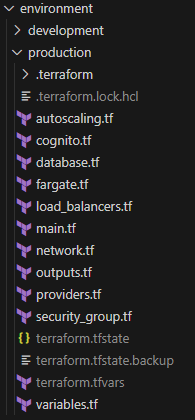
\includegraphics[height=0.4\pdfpageheight]{images/aws-repo-structure.png}
            \caption{Struktura plików Terraform}
            \label{fig:aws-repo-structure}
        \end{figure}

        Pliki \texttt{.tf} zawierają opis zasobów wdrażanych na serwery. Plik \texttt{.tfstate} przechowuje dokładny spis zasobów już wdrożonych wraz z ich unikalnymi identyfikatorami, sekretami, itd. Opis pozostałych plików:
        \begin{itemize}
            \item \texttt{main.tf} - wersje oprogramowania wykorzystywane w projekcie
            \item \texttt{providers.tf} - konfiguracja dostawcy AWS
            \item \texttt{variables.tf} - spis wszystkich zmiennych wraz z ich opisami i niektórymi wartościami domyślnymi
            \item \texttt{terraform.tfvars} - niewersjonowany plik zawierający wartości niektórych zmiennych; przede wszystkim przechowuje sekrety
            \item \texttt{outputs.tf} - zbiór przydatnych wartości wyjściowych, np. nazwa DNS Application Load Balancera
            \item \texttt{network.tf} - zasoby sieciowe: VPC, brama sieciowa, tablice routingu, podsieci
            \item \texttt{security\_groups.tf} - grupy bezpieczeństwa (działają jak zapora ogniowa - ang. firewall) konfigurujące przychodzący i wychodzący ruch sieciowy
            \item \texttt{cognito.tf} - dostawca tożsamości Amazon Cognito i jego konfiguracja
            \item \texttt{load\_balancers.tf} - Application Load Balancer, zasoby nasłuchujące na portach 80, 443 i 8080 oraz grupy celów
            \item \texttt{fargate.tf} - definicje zadań wykonywanych przy pomocy AWS Fargate oraz serwisy które nimi zarządzają
            \item \texttt{autoscaling.tf} - zestaw reguł pozwalających na automatyczne zmniejszanie lub zwiększanie liczby działających instancji modułów (frontendu i backendu)
            \item \texttt{database.tf} - konfiguracja bazy danych RDS
            \item \texttt{sns.tf} - definicja Simple Notification Service (SNS) do wysyłania powiadomień na dany temat do jego subskrybentów
            \item \texttt{lambda.tf} - definiuje funkcję Lambda napisaną w języku TypeScript, uruchamianą okresowo za pomocą alarmów CloudWatch. Funkcja ta pobiera dane z bazy danych i powiadamia subskrybentów, z odpowiednimi rolami zdefiniowanymi w Cognito, na określony temat SNS poprzez e-mail
        \end{itemize}

\end{document}